\documentclass[12pt, aspectratio=169]{beamer}
\usepackage{ctex}          % 支持中文
\usepackage{amsmath, amssymb} % 数学公式
\usepackage{graphicx}      % 图片支持

% 主题设置
\usetheme{Madrid}
\usecolortheme{default}

% 标题信息
\title{第二章：深度学习中的概率论}
\subtitle{精选10题解析}
% \institute{}
\author{《深度学习基础》课程小组}
\date{\today}

\begin{document}
\maketitle

% -----------------------------------------------------------
% 目录页
% -----------------------------------------------------------
\begin{frame}{目录}
    \tableofcontents
\end{frame}

% -----------------------------------------------------------
% 第1页：非传递性骰子 (2.2)
% -----------------------------------------------------------
\section{非传递性骰子}
\begin{frame}[allowframebreaks]{习题 2.2：非传递性骰子 (Efron Dice)}
    \textbf{背景：}
    确定性数字满足传递性 ($x>y, y>z \Rightarrow x>z$)，但随机数不一定。
    
    \textbf{问题描述：}
    考虑四个特殊的立方体骰子（埃夫龙骰子），按循环顺序排列 $A \to B \to C \to D \to A$。
    
    \textbf{任务：}
    \begin{enumerate}
        \item 证明每个骰子掷出比循环中前一个骰子更大数字的概率为 $2/3$。
        \item 解释为何这违反了直觉上的传递性属性。
    \end{enumerate}
    
    \begin{block}{关键点}
        设骰子面值为特定分布，计算 $P(A>B)$, $P(B>C)$, $P(C>D)$, $P(D>A)$ 均等于 $2/3$。
    \end{block}

\newpage 

\begin{figure}[ht]
    \centering
    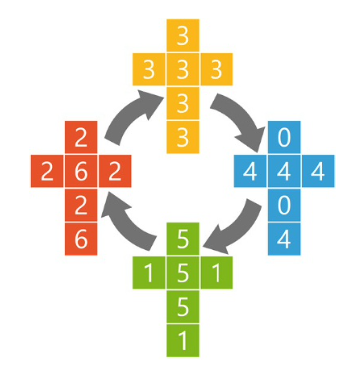
\includegraphics[height=5cm]{efron_dice.png}
    \caption{不确定量的传递性不成立的例子}
    \label{fig:efron_dice}
\end{figure}

\end{frame}

% -----------------------------------------------------------
% 第2页：卷积公式推导 (2.3)
% -----------------------------------------------------------
\section{卷积公式}
\begin{frame}{习题 2.3：独立变量和的分布 (卷积)}
    \textbf{设定：}
    变量 $\mathbf{y} = \mathbf{u} + \mathbf{v}$，其中 $\mathbf{u}, \mathbf{v}$ 相互独立。
    $\mathbf{u} \sim p_{\mathbf{u}}(\mathbf{u})$, $\mathbf{v} \sim p_{\mathbf{v}}(\mathbf{v})$。
    
    \textbf{任务：}
    证明 $\mathbf{y}$ 的概率密度函数为两个分布的卷积：
    
    \begin{equation}
        p(\mathbf{y}) = \int p_{\mathbf{u}}(\mathbf{u})p_{\mathbf{v}}(\mathbf{y} - \mathbf{u}) \,\mathrm{d}\mathbf{u}
    \end{equation}
    
    \begin{block}{提示}
        利用联合分布 $p(\mathbf{u}, \mathbf{v}) = p(\mathbf{u})p(\mathbf{v})$ 和变量代换 $\mathbf{v} = \mathbf{y} - \mathbf{u}$ 进行积分边缘化。
    \end{block}
\end{frame}

% -----------------------------------------------------------
% 第3页：期望与方差分解 (2.11)
% -----------------------------------------------------------
\section{重期望公式}
\begin{frame}{习题 2.11：全期望公式与方差分解}
    \textbf{设定：}
    变量 $x, y$ 具有联合分布 $p(x, y)$。
    
    \textbf{任务：}
    证明以下两个重要恒等式：
    \begin{enumerate}
        \item \textbf{全期望公式 (Law of Iterated Expectations):}
        \[ \mathbb{E}[x] = \mathbb{E}_y [\mathbb{E}_x[x|y]] \]
        
        \item \textbf{方差分解公式 (Law of Total Variance):}
        \[ \text{var}[x] = \mathbb{E}_y [\text{var}_x[x|y]] + \text{var}_y [\mathbb{E}_x[x|y]] \]
    \end{enumerate}
    
    \begin{alertblock}{物理意义}
        总方差 = 组内方差的期望 + 组间方差（期望的方差）。
    \end{alertblock}
\end{frame}

% -----------------------------------------------------------
% 第4页：高斯分布的二阶矩 (2.16)
% -----------------------------------------------------------
\section{高斯分布的二阶矩}
\begin{frame}{习题 2.16：高斯采样的相关性}
    \textbf{设定：}
    $x_n, x_m$ 是从 $\mathcal{N}(\mu, \sigma^2)$ 中独立采样的数据点。
    已知 $\mathbb{E}[x^2]=\mu^2+\sigma^2$。
    
    \textbf{任务：}
    证明两点乘积的期望为：
    \begin{equation}
        \mathbb{E}\left[x_{n} x_{m}\right]=\mu^{2}+I_{n m} \sigma^{2}
    \end{equation}
    其中 $I_{nm}$ 为单位矩阵元素 ($n=m$ 时为1，否则为0)。
    
    \begin{block}{分析思路}
        \begin{itemize}
            \item 当 $n \neq m$：独立，$\mathbb{E}[x_n x_m] = \mathbb{E}[x_n]\mathbb{E}[x_m] = \mu^2$。
            \item 当 $n = m$：$\mathbb{E}[x_n^2] = \text{var}[x] + (\mathbb{E}[x])^2 = \sigma^2 + \mu^2$。
        \end{itemize}
    \end{block}
\end{frame}

% -----------------------------------------------------------
% 第5页：概率密度的变量变换 (2.19)
% -----------------------------------------------------------
\section{概率密度的变量变换}
\begin{frame}{习题 2.19：任意密度的生成变换}
    \textbf{理论：}
    利用变量变换公式 $p_y(y) = p_x(x) \left| \frac{dx}{dy} \right|$。
    
    \textbf{任务：}
    \begin{enumerate}
        \item 证明任何目标密度 $p(y)$ 都可以通过对固定密度 $q(x)$ (处处非零) 进行单调变换 $y=f(x)$ 获得。
        \item 写出 $f(x)$ 满足的微分方程。
        \item 绘制示意图说明密度如何被拉伸或压缩。
    \end{enumerate}
    
    \begin{equation}
        p(f(x)) \cdot f'(x) = q(x) \quad \Rightarrow \quad f'(x) = \frac{q(x)}{p(f(x))}
    \end{equation}
\end{frame}

% -----------------------------------------------------------
% 第6页：雅可比矩阵计算 (2.20)
% -----------------------------------------------------------
\section{非线性变换的雅可比矩阵}
\begin{frame}{习题 2.20：非线性变换的雅可比矩阵}
    \textbf{变换定义：}
    \begin{align}
        y_1 &= x_1 +\tanh(5x_1) \\
        y_2 &= x_2 +\tanh(5x_2) +\frac{x_1^3}{3}
    \end{align}
    
    \textbf{任务：}
    计算该变换的雅可比矩阵 $\mathbf{J}$ 的元素 $J_{ij} = \frac{\partial y_i}{\partial x_j}$。
    
    \begin{block}{解答结构}
        \[
        \mathbf{J} = \begin{pmatrix} 
        \frac{\partial y_1}{\partial x_1} & \frac{\partial y_1}{\partial x_2} \\
        \frac{\partial y_2}{\partial x_1} & \frac{\partial y_2}{\partial x_2}
        \end{pmatrix} = \begin{pmatrix} 
        1 + 5\text{sech}^2(5x_1) & 0 \\
        x_1^2 & 1 + 5\text{sech}^2(5x_2)
        \end{pmatrix}
        \]
    \end{block}
\end{frame}

% -----------------------------------------------------------
% 第7页：高斯分布的熵 (2.25)
% -----------------------------------------------------------
\section{高斯分布的熵}
\begin{frame}{习题 2.25：单变量高斯分布的熵}
    \textbf{定义：}
    微分熵 $H[x] = -\int p(x) \ln p(x) dx$。
    
    \textbf{任务：}
    证明均值为 $\mu$、方差为 $\sigma^2$ 的高斯分布 $N(\mu,\sigma^2)$ 的熵为：
    
    \begin{equation}
        H[x]=\frac{1}{2}\left(1+\ln (2\pi\sigma^2)\right)
    \end{equation}
    
    \begin{alertblock}{结论意义}
        高斯分布的熵仅取决于方差 $\sigma^2$，与均值 $\mu$ 无关。方差越大，不确定性越高。
    \end{alertblock}
\end{frame}

% -----------------------------------------------------------
% 第8页：KL 散度计算 (2.27)
% -----------------------------------------------------------
\section{KL 散度计算}
\begin{frame}{习题 2.27：两个高斯分布的 KL 散度}
    \textbf{设定：}
    $p(x)=\mathcal{N}(x | \mu, \sigma^{2})$， $q(x)=\mathcal{N}(x | m, s^{2})$。
    
    \textbf{任务：}
    计算 Kullback-Leibler 散度 $KL(p || q)$：
    \[ KL(p||q) = \int p(x) \ln \frac{p(x)}{q(x)} dx \]
    
    \begin{block}{最终公式}
        \[
        KL(p||q) = \frac{1}{2} \left( \ln\frac{s^2}{\sigma^2} + \frac{\sigma^2 + (\mu-m)^2}{s^2} - 1 \right)
        \]
    \end{block}
    \textbf{提示：}分别计算 $\mathbb{E}_p[\ln p(x)]$ 和 $\mathbb{E}_p[\ln q(x)]$。
\end{frame}

% -----------------------------------------------------------
% 第9页：联合熵与独立性 (2.29)
% -----------------------------------------------------------
\section{联合熵与独立性}
\begin{frame}{习题 2.29：联合熵的不等式}
    \textbf{设定：}
    变量 $\mathbf{x}, \mathbf{y}$ 具有联合分布 $p(\mathbf{x}, \mathbf{y})$。
    
    \textbf{任务：}
    证明微分熵满足次可加性：
    \begin{equation}
        \mathrm{H}[\mathbf{x}, \mathbf{y}] \leqslant \mathrm{H}[\mathbf{x}]+\mathrm{H}[\mathbf{y}]
    \end{equation}
    并证明当且仅当 $\mathbf{x}$ 和 $\mathbf{y}$ \textbf{统计独立} 时取等号。
    
    \begin{alertblock}{证明思路}
        利用互信息 $I(\mathbf{x};\mathbf{y}) = H(\mathbf{x}) + H(\mathbf{y}) - H(\mathbf{x}, \mathbf{y}) \geqslant 0$。
        互信息为零等价于独立。
    \end{alertblock}
\end{frame}

% -----------------------------------------------------------
% 第10页：线性变换下的熵变 (2.30)
% -----------------------------------------------------------
\section{线性变换对熵的影响}
\begin{frame}{习题 2.30：线性变换对熵的影响}
    \textbf{设定：}
    $\mathbf{x} \sim p(\mathbf{x})$，进行非奇异线性变换 $\mathbf{y}=\mathbf{A} \mathbf{x}$。
    
    \textbf{任务：}
    证明新变量的熵为：
    \begin{equation}
        \mathrm{H}[\mathbf{y}]=\mathrm{H}[\mathbf{x}]+\ln | \operatorname{det} \mathbf{A} |
    \end{equation}
    
    \begin{block}{直观理解}
        \begin{itemize}
            \item 行列式 $|\det \mathbf{A}|$ 代表变换引起的体积伸缩率。
            \item 体积扩大 $\rightarrow$ 分布更分散 $\rightarrow$ 熵增加。
            \item 若 $\mathbf{A}$ 为正交矩阵 (旋转)，行列式为1，熵不变。
        \end{itemize}
    \end{block}
\end{frame}

\end{document}
